\chapter{Ход работы}
\label{ch:chap2}

\section{\textbf{Поллячек и Хинчин}}

Феликс Поллячек (1892–1981) — австрийский математик и инженер. Один из первых исследовал очереди и СМО, разработал анализ 
характеристик M/G/1-систем. Ввёл формулу для среднего числа заявок в системе с произвольным временем обслуживания. \\

Александр Хинчин (1894–1959) - советский математик. Совместно с Поллячек разработал аналитические формулы для M/G/1.

\section{\textbf{Ход работы}}

Зададим базовые параметры СМО - интенсивность поступления заявок и интенсивность обработки. Высчитаем мат.ожидание и дисперсию 
экспоненциального распределения, которое понадобится для M/M/1. Высчитаем коэффициент загруженности системы.

\begin{lstlisting}
%define params
lambda = 5;
u = 15;

% E and D for exp distr
E = 1/lambda;
D = 1/lambda^2;

% coef of using sysytem
p_v = lambda / u;
\end{lstlisting}

Для расчетов параметров для системы M/G/1 я выбрал гамма распределение, оно характеризуется параметрами a и k

\begin{figure}[H]
    \centering
    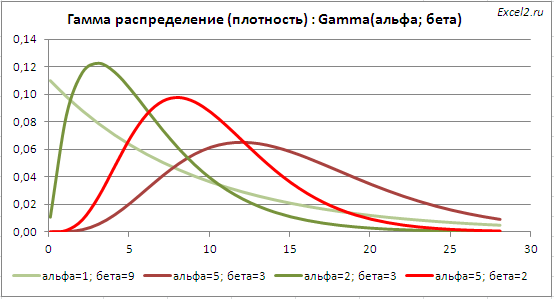
\includegraphics[width=1.0\textwidth]{gamma.png}
    \caption{Гамма-распределение}
\end{figure}

a - коэффициент формы, благодаря ему распределение становится более симметричным и меньше скошено вправо или влево (при увеличении).
b - коэффициент масштабирования, он растягивает распределение, среднее и дисперсия увеличиваются. \\

Чтобы правильно подобрать a и b нужно решить систему уравений

\[
\begin{aligned}
ab = 0.2 \\
ab^2 = 0.04
\end{aligned}
\]
Отсюда a = 1, b = 0.2. Теперь зададим распределение 

\begin{lstlisting}
%params for time serving distr (gamma)
a = 1;
b = 0.2;
N_i = 250;

%exp distr
exp_distr = exprnd(E, 1, N_i);

%gamma distr
MG1_tn = gamrnd(a, b, 1, N_i);

\end{lstlisting}

Необходимо построить зависимости СМО M/G/1 от загруженности системы p и нормированной дисперсии времени обслуживания $c^2$. Зададим
набор значений вручную. 0 < p < 1. Далее в цикле высчитываем метрики и выводим на график.

\begin{lstlisting}
%vector of var
var = [0, 1, 10, 20, 30, 40, 50, 60, 70, 80, 90, 100];
p_v = [0.1, 0.2, 0.3, 0.4, 0.5, 0.6, 0.7, 0.8, 0.9];
p_count = length(p_v);

N_q = zeros(p_count, 1);
N = zeros(p_count, 1);
W = zeros(p_count, 1); 
T = zeros(p_count, 1);

for i = 1: length(p_v)
    stats =  MG1_param(MG1_tn, 0, p_v(i));
    N_q(i) = stats.N_q;
    N(i) = stats.N;
    W(i) = stats.W;
    T(i) = stats.T;
end

figure;
subplot(4, 1, 1);
plot(p_v, N_q);
xlabel("p");
ylabel("N_q");
title("Среднее число заявок в СМО M/G/1");
subplot(4, 1, 2);
plot(p_v, N);
xlabel("p");
ylabel("N");
title("Среднее число заявок в СМО M/G/1");
subplot(4, 1, 3);
plot(p_v, W);
xlabel("p");
ylabel("N");
title("Среднее время ожидания для M/G/1");
subplot(4, 1, 4);
plot(p_v, T);
xlabel("p");
ylabel("N");
title("Среднее время пребывания требования в системе для M/G/1");
\end{lstlisting}

Для остальных систем код идентичен. \\

Код для высчитывания метрик разных СМО

\begin{lstlisting}
function stats = MG1_param(tn, c, p)
    %N_q - avg queue len
    %N - avg tasks count in system
    %W - avg waiting time 
    %T - avg time task into system
    %t_n - set of time serving

    %avg time serving
    avg_tn = mean(tn);

    %compute params
    stats.N_q = p^2 * (1 + c) / (2*(1-p));
    stats.N = p + stats.N_q;
    stats.W = p * avg_tn * (1 + c) / (2*(1-p));
    stats.T = avg_tn + stats.W;

end

function stats = MD1_param(t, p)
    %N_q - avg queue len
    %N - avg tasks count in system
    %W - avg waiting time 
    %T - avg time task into system
    %t - time serving

    %compute params
    stats.N_q = p^2 * 1 / (2*(1-p));
    stats.N = p + stats.N_q;
    stats.W = p * t / (2*(1-p));
    stats.T = t*(1 - p) / (2 * (1 - p));
end

function stats = MM1_param(tn, p)
    %N_q - avg queue len
    %N - avg tasks count in system
    %W - avg waiting time 
    %T - avg time task into system
    %t_n - set of time serving

    %avg time serving
    avg_tn = mean(tn);

    %compute params
    stats.N_q = p^2/(1-p);
    stats.N = p / (1 - p);
    stats.W = stats.N * avg_tn;
    stats.T = avg_tn / (1-p);

end
\end{lstlisting}

Результаты:

\begin{figure}[H]
    \centering
    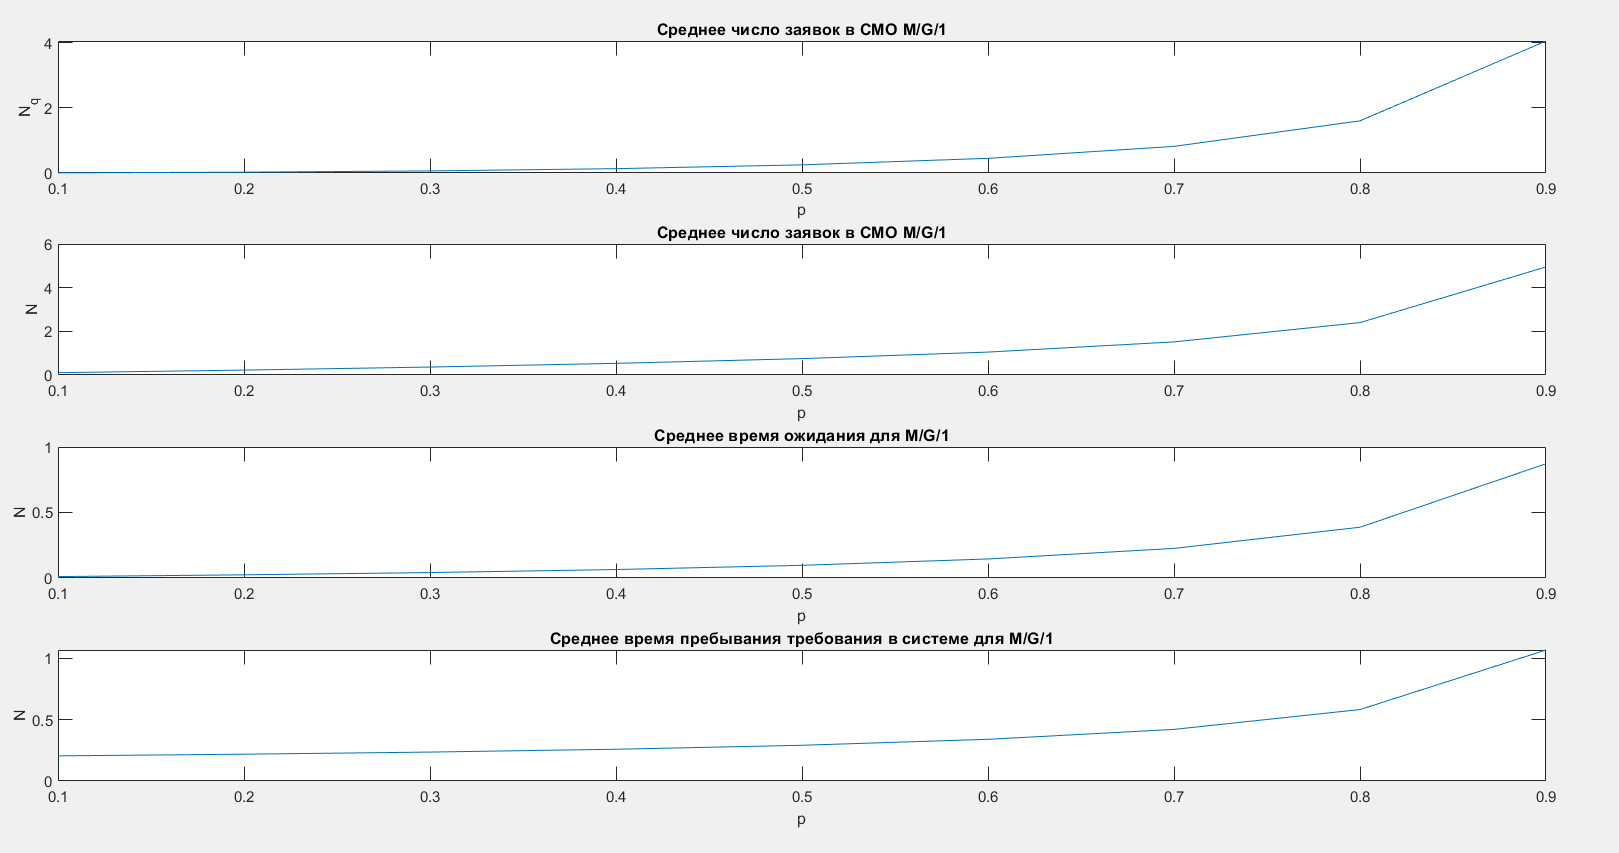
\includegraphics[width=1.0\textwidth]{mg1p.png}
    \caption{Зависимость параметров СМО M/G/1 от загруженности}
\end{figure}

\begin{figure}[H]
    \centering
    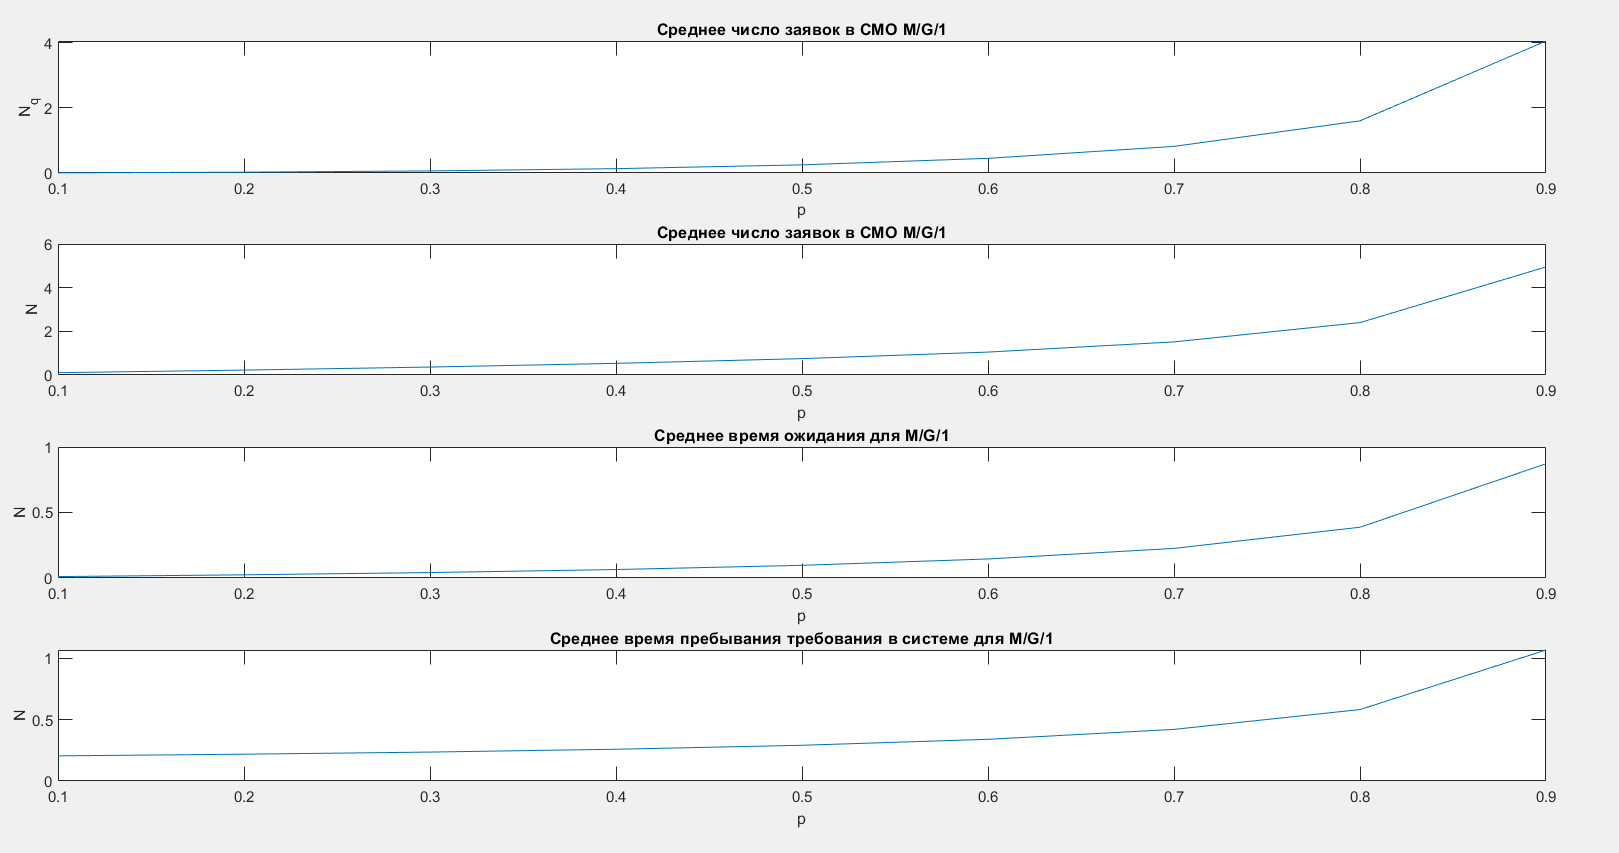
\includegraphics[width=1.0\textwidth]{mg1p.png}
    \caption{Зависимость параметров СМО M/G/1 от дисперсии времени обработки}
\end{figure}

\begin{figure}[H]
    \centering
    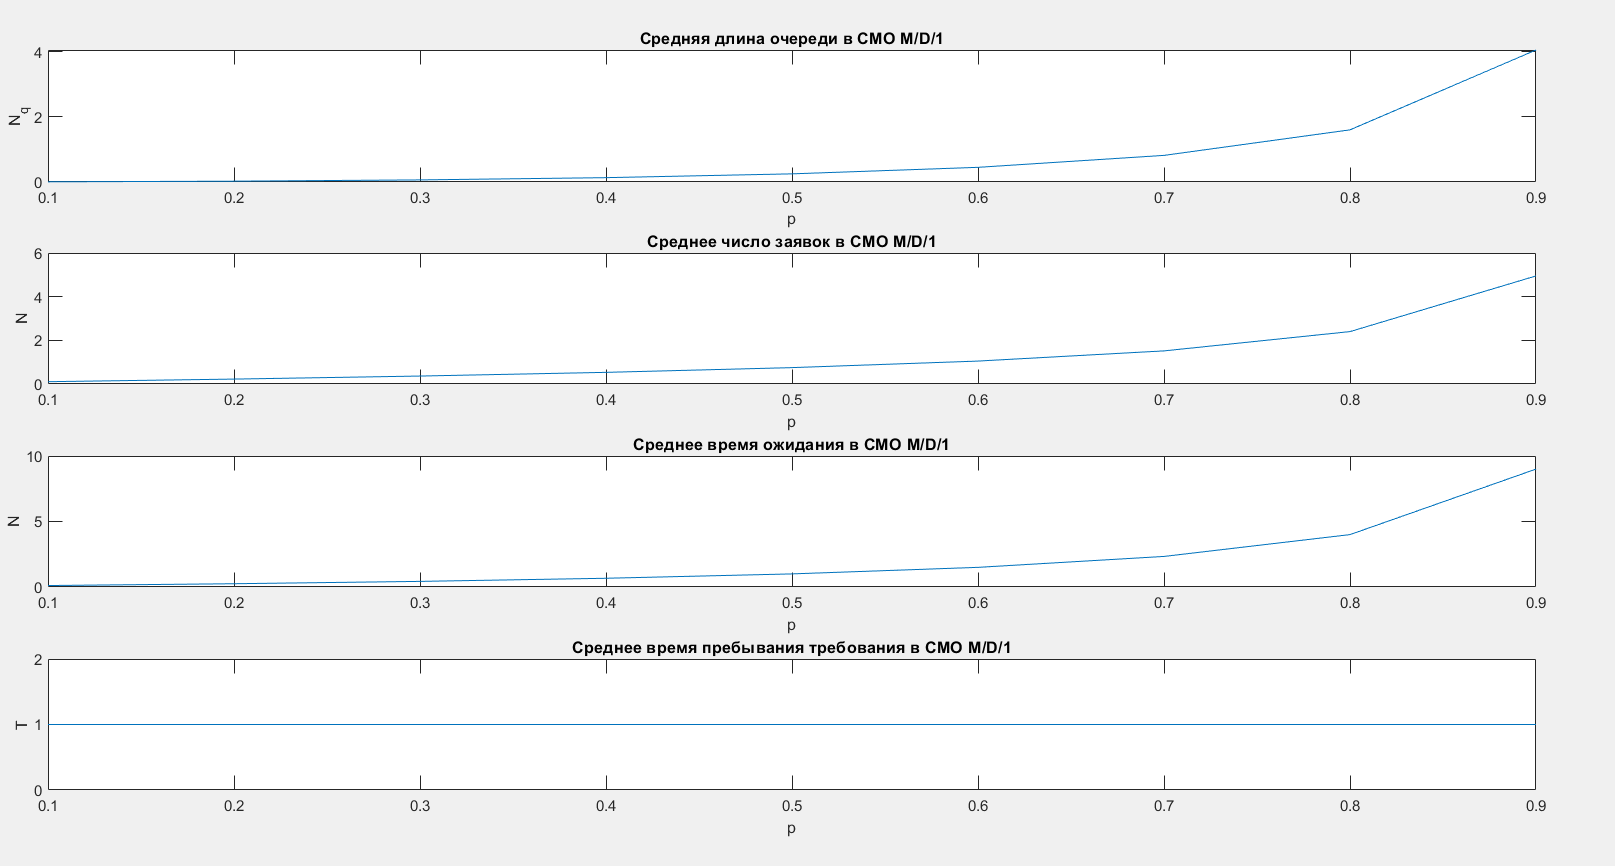
\includegraphics[width=1.0\textwidth]{md1.png}
    \caption{Зависимость параметров СМО M/D/1 от загруженности системы}
\end{figure}

\begin{figure}[H]
    \centering
    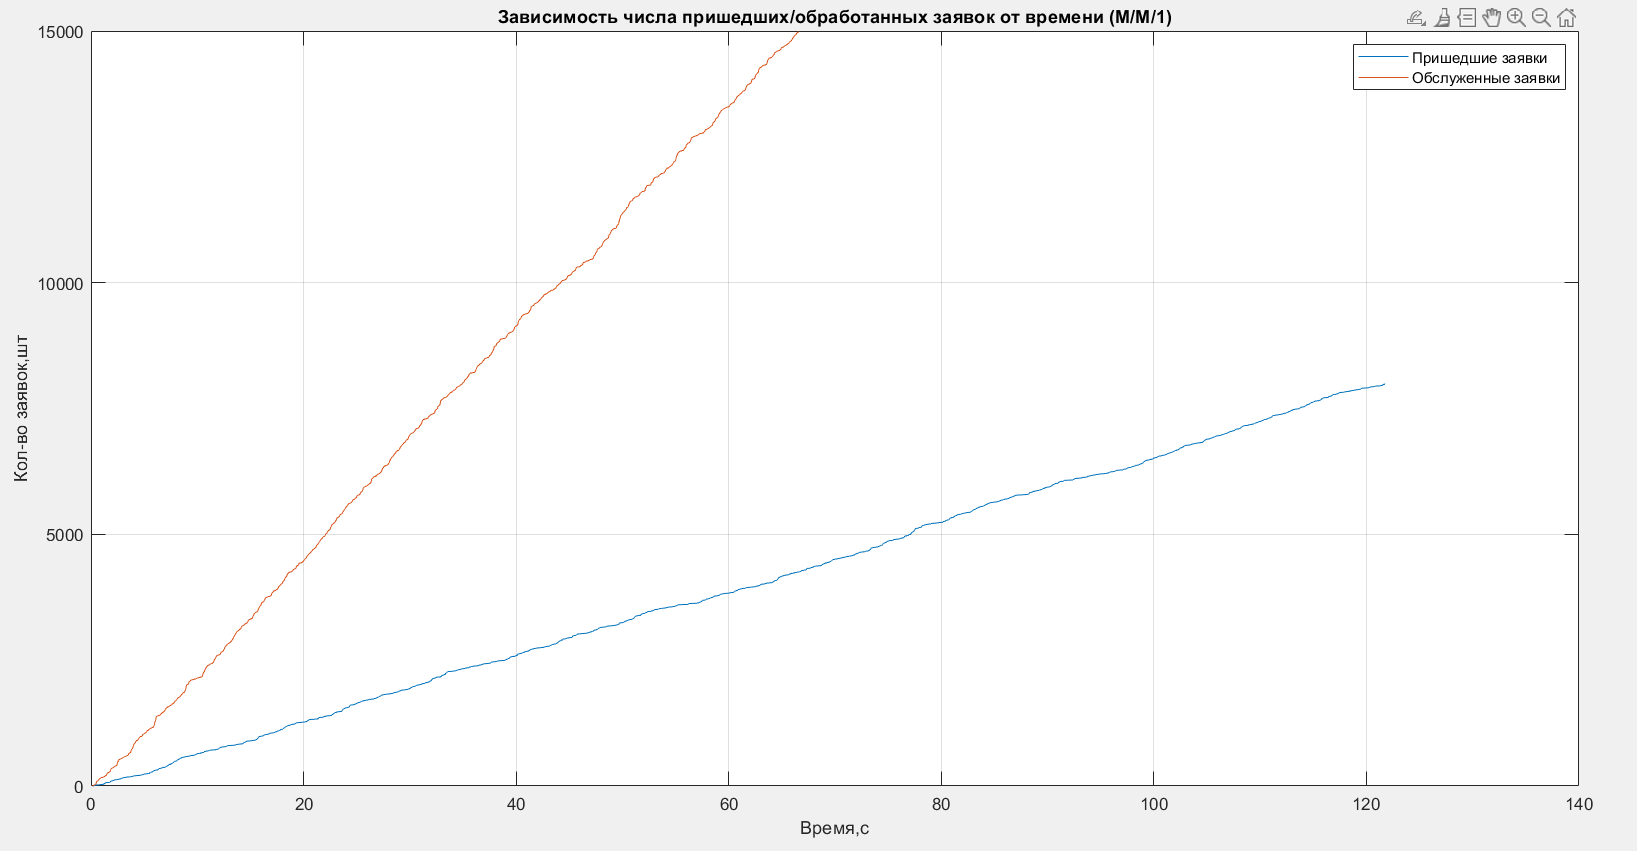
\includegraphics[width=1.0\textwidth]{mm1.png}
    \caption{Зависимость параметров СМО M/M/1 от загруженности системы}
\end{figure}

По результатам можем заметить, что метрики всех видов рассмотренных СМО экспоненциально растут при росте загруженности системы, кроме системы
M/D/1, потому что у нее время обработки детерминированно (константа). Система M/G/1 зависит от нормированной дисперсии времени обработки линейно.

\section{\textbf{Контрольные вопросы}}

\begin{figure}[H]
    \centering
    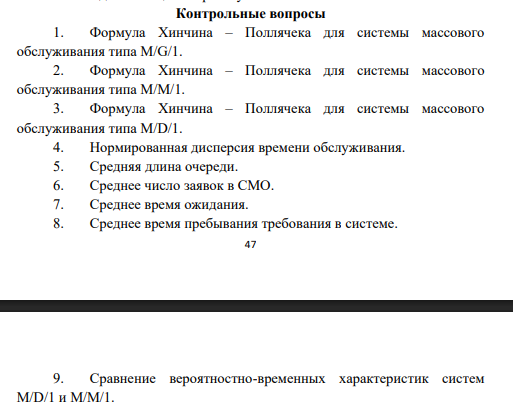
\includegraphics[width=1.0\textwidth]{cas.png}
    \caption{Контрольные вопросы}
\end{figure}

\begin{figure}[H]
    \centering
    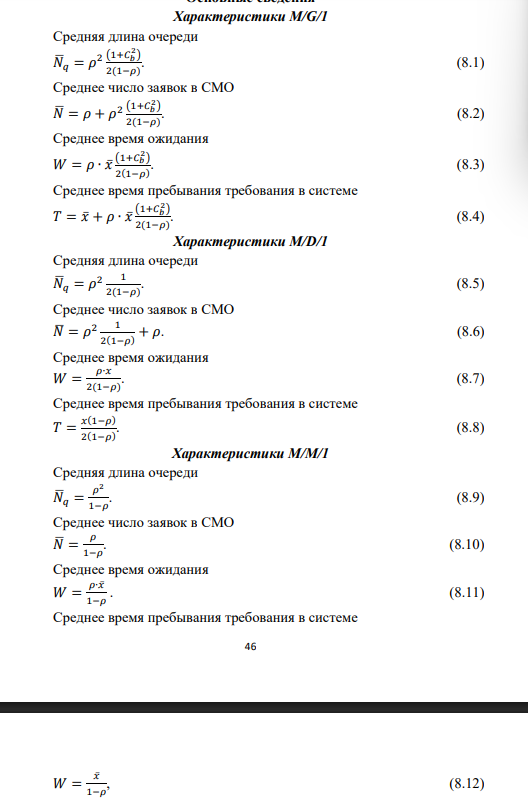
\includegraphics[width=1.0\textwidth]{ca1.png}
    \caption{Вопросы 1-3}
\end{figure}

4. Нормированная дисперсия времени обслуживания - дисперсия времени обслуживания, нормированная по среднему времени обработки заявки: 
$c^2 = \frac{\sigma^2}{\dot{x}^2}$. \\

5. Средняя длина очереди - кол-во заявок, ожидающих свою обработку в очереди. \\

6. Среднее число заявок в СМО - кол-во заявок, которое находится в очереди и обрабатывается. \\

7. Среднее время ожидания - то время, которое заявка ожидает в очереди перед обработкой. \\

8. Среднее время пребывания требования в системе - то время, которое заявка находится в системе с момента ее поступления в нее до
момента полной обработки. \\

9. Системы M/D/1 и M/M/1 отличаются временем обработки заявок. В M/M/1 время обработки распределено по экспоненциальному закону,
а в M/D/1 время обработки - константа. Сисетма M/D/1 - идеализированная система, где время обработки никак не зависит от нагрузки,
что в реальности невозможно.



\endinput
